% ============================================================
%  cvstyle.tex -- shared preamble/macros for Zihao-Eric GUO's CV
%  Recreates the two-column "sidebar + timeline" Word template
%  used in CV_doc/*.docx (one page, A4).
%  Included by CV_Zihao_EN.tex / CV_Zihao_FR.tex / CV_Zihao_CH.tex
% ============================================================

\documentclass[10pt,a4paper]{article}

\usepackage[T1]{fontenc}
\usepackage[utf8]{inputenc}
\usepackage{carlito}                 % Calibri-metric-compatible font
\renewcommand{\familydefault}{\sfdefault}

\usepackage[paperwidth=210mm,paperheight=297mm,margin=0mm]{geometry}
\usepackage[absolute,overlay]{textpos}
\usepackage{eso-pic}
\usepackage{tikz}
\usetikzlibrary{shadows,shapes.geometric}
\usepackage{xcolor}
\usepackage{array}
\usepackage{ragged2e}
\usepackage{enumitem}
\usepackage{fontawesome5}
\usepackage{graphicx}
\usepackage[hidelinks]{hyperref}

\pagestyle{empty}
\setlength{\parindent}{0pt}
\renewcommand{\arraystretch}{1}

% ---------------- colours (sampled from the original docx) ----------------
\definecolor{cvblue}{HTML}{017BAA}   % banner / skill box / icon badges / bars
\definecolor{cvbluedark}{HTML}{004F6E}
\definecolor{cvgray}{HTML}{F3F3F3}   % sidebar + section-header bar
\definecolor{cvlink}{HTML}{0563C1}   % hyperlink blue
\definecolor{cvdot}{HTML}{0070C0}    % bullet / timeline rule blue
\definecolor{cvrule}{HTML}{BFBFBF}   % timeline grey rule
\definecolor{cvtext}{HTML}{000000}

\hypersetup{colorlinks=true, urlcolor=cvlink, linkcolor=cvlink}

% ---------------- text grid -------------------------------------------------
\setlength{\TPHorizModule}{1mm}
\setlength{\TPVertModule}{1mm}
\textblockorigin{0mm}{0mm}

% ---------------- layout dimensions -----------------------------------------
\newlength{\sidew}    \setlength{\sidew}{61mm}    % sidebar width
\newlength{\sidepad}  \setlength{\sidepad}{4mm}   % sidebar inner padding
\newlength{\mainx}    \setlength{\mainx}{64mm}    % right column x-origin
\newlength{\mainw}    \setlength{\mainw}{139mm}   % right column width

\newlength{\sideinnerw}
\setlength{\sideinnerw}{\sidew}
\addtolength{\sideinnerw}{-2\sidepad}

\newlength{\cvdatew}  \setlength{\cvdatew}{24mm}
\newlength{\cvgutter} \setlength{\cvgutter}{4mm}
\newlength{\cvcontw}
\setlength{\cvcontw}{\mainw}
\addtolength{\cvcontw}{-\cvdatew}
\addtolength{\cvcontw}{-\cvgutter}

% ---------------- full-bleed sidebar background -----------------------------
\AddToShipoutPictureBG*{%
  
\begin{tikzpicture}[remember picture,overlay,x=1mm,y=-1mm]
    \fill[cvgray] (0,0) rectangle (61,297);
  \end{tikzpicture}%
}

% ---------------- generic helpers -------------------------------------------

% small filled dot bullet (sidebar contact rows / language rows)
\newcommand{\cvdotmark}{\textcolor{cvdot}{\Large\textbullet}}

% language proficiency bar: #1 = fill fraction in [0,1]
\newcommand{\langbar}[1]{%
  \begin{tikzpicture}[x=1mm,y=1mm]
    \def\w{45}\def\h{3.2}
    \draw[black, line width=0.6pt, rounded corners=0.7pt] (0,0) rectangle (\w,\h);
    \fill[cvblue] (0.18,0.18) rectangle ({#1*\w-0.18},{\h-0.18});
  \end{tikzpicture}%
}

% sidebar section title (bold black, no bar)
\newcommand{\sidetitle}[1]{%
  \par\vspace{1mm}\textbf{\Large #1}\par\vspace{1.3mm}%
}

% compact sidebar education entry: #1=institution #2=dates/location #3=description
\newcommand{\sideedu}[3]{%
  \cvdotmark\ \textbf{\normalsize #1}\par\vspace{0.6mm}
  {\footnotesize\textit{\textcolor{black!65}{#2}}}\par\vspace{0.6mm}
  {\footnotesize\itshape #3}\par%
}

% section badge + heading bar for the main column
% #1 = fontawesome icon command   #2 = heading text
\newcommand{\cvsection}[2]{%
  \par\vspace{6mm}\noindent%
  \begin{tikzpicture}[baseline=-3.2mm,x=1mm,y=1mm]
    \node[fill=cvblue, rounded corners=1.2pt, minimum width=8mm, minimum height=8mm, inner sep=0pt]
      (badge) at (4,-4) {\textcolor{white}{\fontsize{11}{11}\selectfont #1}};
    \fill[cvblue] (1.2,-7.6) -- (3,-8.6) -- (3,-7.6) -- cycle; % small tail
  \end{tikzpicture}%
  \hspace{1.5mm}%
  \colorbox{cvgray}{\makebox[127mm][l]{\rule{0pt}{3.6mm}\textbf{\Large \MakeUppercase{#2}}}}%
  \par\vspace{2.8mm}%
}

% timeline row: #1=date (bold)  #2=location (italic)  #3=main content
\newcommand{\cvrow}[3]{%
  \noindent
  \begin{tabular}{@{}p{\cvdatew}!{\color{cvrule}\vrule width 0.8pt}p{\cvcontw}@{}}
  \begin{minipage}[t]{\cvdatew}\raggedright\textbf{#1}\par\vspace{0.8mm}\textit{\textcolor{black!65}{#2}}\end{minipage}
  & \hspace{3mm}\begin{minipage}[t]{\cvcontw}#3\end{minipage}\\
  \end{tabular}\par\vspace{6mm}%
}

% continuation row (no date/location repeated, just the rule + content)
\newcommand{\cvcont}[1]{%
  \noindent
  \begin{tabular}{@{}p{\cvdatew}!{\color{cvrule}\vrule width 0.8pt}p{\cvcontw}@{}}
  \mbox{} & \hspace{3mm}\begin{minipage}[t]{\cvcontw}#1\end{minipage}\\
  \end{tabular}\par%
}

\newcommand{\kw}[1]{\underline{\texttt{\footnotesize #1}}}

\newcommand{\entrydate}[1]{\hspace{3mm plus 1fill}\textit{\underline{#1}}}

\newlist{cvitemize}{itemize}{1}
\setlist[cvitemize]{leftmargin=4mm, itemsep=0pt, topsep=1pt, parsep=0pt, label=\textbullet}

\newlist{sideitemize}{itemize}{1}
\setlist[sideitemize]{leftmargin=3mm, itemsep=0.5pt, topsep=1pt, parsep=0pt, label=\textbullet}


\begin{document}

% =========================== SIDEBAR (left) ===========================
\begin{textblock*}{\sideinnerw}(\sidepad,3mm)
\begin{minipage}[t]{\sideinnerw}
{\centering
\begin{tikzpicture}
  \clip (0,0) circle (16mm);
  \node[anchor=center] at (0,0) {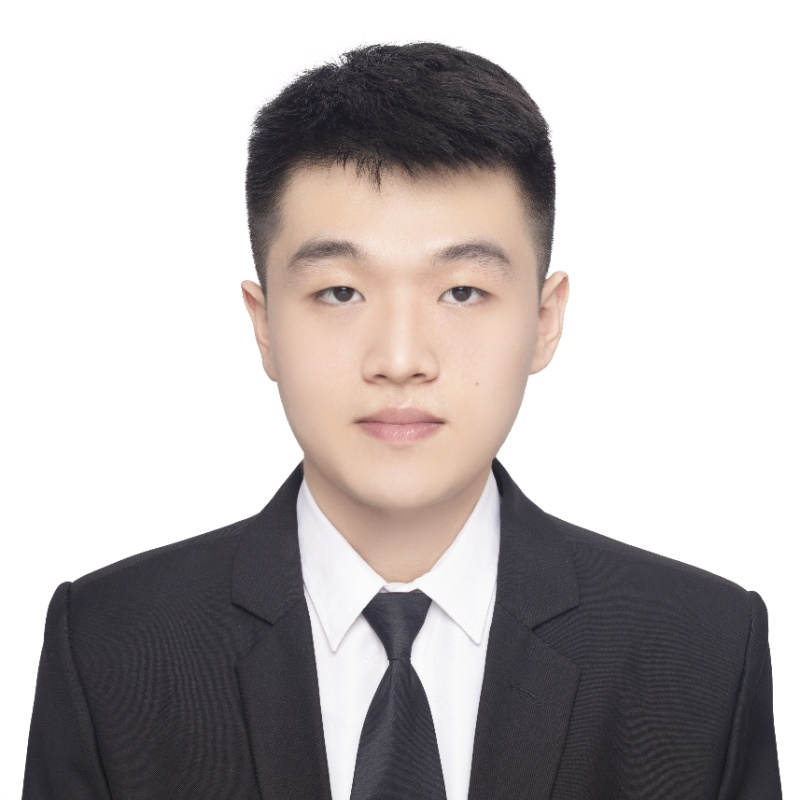
\includegraphics[width=34mm]{assets/photo.jpg}};
\end{tikzpicture}
\par}

\vspace{2mm}
{\centering{\LARGE\textbf{Zihao-Eric GUO}}\par}
\vspace{2mm}

{\normalsize
\faEnvelope\ \href{mailto:zihao-eric.guo@ip-paris.fr}{zihao-eric.guo@ip-paris.fr}\par\vspace{1mm}
\faPhone\ +33 (0)765241550\par\vspace{1mm}
\faMapMarker\ Paris, France\par\vspace{1mm}
\faTrophy\ Kaggle Expert\par\vspace{1mm}
\faHome\ \href{https://zihao-guo.github.io/}{Ma page perso}\par
}

\vspace{3mm}
\sidetitle{FORMATION}
\sideedu{Institut Polytechnique de Paris (\href{https://www.ip-paris.fr/}{IPP})}{Depuis 11/2023 -- Paris, France}{Préservation des performances des graphes en environnement exogènement perturbé - Date de fin: \textbf{\underline{déc. 2026}}}
\vspace{1.5mm}
\sideedu{École Centrale de Nantes (\href{https://www.ec-nantes.fr/english-version}{ECN})}{09/2021 -- 09/2023 -- Nantes, France}{Diplôme d'ingénieur généraliste (\textbf{MSc}) - option maths appliquées}
\vspace{1.5mm}
\sideedu{Université de Picardie Jules Verne (\href{https://www.u-picardie.fr/}{UPJV})}{09/2017 -- 07/2021 -- Amiens, France}{Licence (\textbf{BSc}), optimisation}

\vspace{3mm}
\sidetitle{COMPÉTENCES IT}
\tikz\node[fill=cvblue, text=white, rounded corners=2pt, text width=\sideinnerw-4mm, inner sep=2.2mm]{\small Python, R, C/C++, NoSQL, MATLAB, Power BI, Gurobi/Cplex, \mbox{CUDA (vibe coding)}};

\vspace{3mm}
\sidetitle{LANGUES}
{\centering\normalsize
\cvdotmark\ \textbf{Chinois} : langue maternelle\par\vspace{0.6mm}
\langbar{0.95}\par\vspace{1mm}
\cvdotmark\ \textbf{Anglais} : courant (GRE 326)\par\vspace{0.6mm}
\langbar{0.82}\par\vspace{1mm}
\cvdotmark\ \textbf{Français} : courant (DALF C1)\par\vspace{0.6mm}
\langbar{0.72}\par
}

\vspace{3mm}
\sidetitle{INTÉRÊTS}
{\centering\textcolor{cvblue}{\LARGE\faBookOpen\ \faBasketballBall\ \faFutbol}\ \cvflower\par}

\vspace{3mm}
\sidetitle{Atouts}
{\normalsize\itshape
\begin{sideitemize}
\item Esprit d'équipe ;
\item Indépendance et adaptabilité ;
\item Forte capacité d'apprentissage.
\end{sideitemize}
}
\end{minipage}
\end{textblock*}

% =========================== MAIN COLUMN (right) ===========================
\begin{textblock*}{\mainw}(\mainx,3mm)

% ---- banner ----

\begin{tikzpicture}[x=1mm,y=-1mm]
  \node[fill=black!15, rounded corners=3pt, minimum width=143mm, minimum height=27mm, inner sep=0pt] at (71.5,14.8) {};
  \shade[shading=axis, left color=cvblue, right color=cvbluedark, shading angle=-25,
        rounded corners=3pt] (0,0) rectangle (143,27);
  \node[anchor=north west, text=white, text width=95mm, align=left, inner sep=0pt] at (5,4)
    {\faIdBadge\ Pré-doc à l'Institut Polytechnique de Paris\par\vspace{0.8mm}Intéressé: optimisation stochastique, programmation mathématique};
  \node[anchor=north east, text=white] at (138,19.5)
    {\large\textbf{Ingénieur IA | Ingénieur algorithmes | Data scientist}};
  \node[fill=white, minimum width=8mm, minimum height=8mm, inner sep=0pt] at (117,7) {\href{https://www.linkedin.com/in/zihao-éric-g-850167211/}{\textcolor{cvblue}{\large\faLinkedin}}};
  \node[fill=white, minimum width=8mm, minimum height=8mm, inner sep=0pt] at (128,7) {\href{https://github.com/zeio99}{\textcolor{black}{\large\faGithub}}};
\end{tikzpicture}
\vspace{-2mm}
\fontsize{12}{14.5}\selectfont

% ---- EXPÉRIENCE PRO ----
\cvsection{\faFlag}{Expérience pro}

\cvrow{2025}{Shanghai,\\ \textbf{\itshape Chine}}{%
\textbf{Stage -- Ing. algorithmes (\href{https://www.huawei.com/fr/}{Huawei})}\par
{\normalsize\itshape\textcolor{black!65}{08/2025 -- 11/2025}}\par
\begin{cvitemize}
\item Développement d'un cadre contrastif multimodal nuage de points-canal pour la prédiction du canal, avec un algorithme d'allocation non contiguë améliorant l'allocation continue RIV.
\end{cvitemize}
Mots-clés : \kw{apprentissage contrastif multimodal, optimisation}}

\cvrow{2023}{Cambridge,\\ \textbf{\itshape Royaume-Uni}}{%
\textbf{Stage -- Assistant de recherche en biostatistique (\href{https://en.wikipedia.org/wiki/European_Bioinformatics_Institute}{EMBL-EBI})}\par
{\normalsize\itshape\textcolor{black!65}{04/2023 -- 09/2023}}\par
\begin{cvitemize}
\item Sujet : « Simuler l'évolution des génomes sur de grands arbres phylogénétiques à branches courtes »
\end{cvitemize}
Mots-clés : \kw{R/Python, échantillonnage, cluster, bash(UNIX)}}

\cvrow{2022}{Paris,\\ \textbf{\itshape France}}{%
\textbf{Stage -- Data Engineer (\href{https://www.ifpenergiesnouvelles.com/}{IFPEN})}\par
{\normalsize\itshape\textcolor{black!65}{04/2022 -- 08/2022}}\par
\begin{cvitemize}
\item Analyse des données de validation des badges de trafic et création d'un tableau de bord.
\item Comparaison des données issues du modèle de trafic (MATSim) pour analyser les erreurs.
\item Utilisation de modèles temporels (Sarimax, NeuralProphet...) pour corriger les statistiques par prédiction.
\end{cvitemize}
Mots-clés : \kw{Django, HTML/CSS, MongoDB, Git, PyTorch, Statsmodels}}

% ---- RECHERCHE SCIENTIFIQUE ----
\cvsection{\faTrophy}{Recherche scientifique}

\cvsubtitle{Publications sélectionnées}
\cvfull{%
\textbf{Classification de textes CNN par recuit simulé}\par
{\normalsize\itshape\textcolor{black!65}{ACM - International Conference Proceeding Series (ISBN: 978-1-4503-8432-2)}}\par
\vspace{1mm}
\textbf{Accessibilité du rail urbain via refonte du réseau de bus}\par
{\normalsize\itshape\textcolor{black!65}{Transportation Research Board (TRB) 104th Annual Meeting}}\par
\vspace{1mm}
\textbf{Variations de taux et erreurs récurrentes en phylogénétique}\par
{\normalsize\itshape\textcolor{black!65}{Nature Methods}}\par
\vspace{1.5mm}
\centerline{\normalsize Voir plus de publications sur mon \href{https://scholar.google.com/citations?view_op=list_works&hl=en&hl=en&user=gMy-9XEAAAAJ}{Google Scholar profile}.}}

\cvsubtitle{Recherche}
\cvfull{%
\textbf{Apprentissage multitâche pour les réseaux bayésiens}\par
{\normalsize\itshape\textcolor{black!65}{Oct. 2022 -- avr. 2023, Nantes, France -- Laboratoire des Sciences du Numérique de Nantes (LS2N)}}\par
Mots-clés : \kw{C++, réseaux bayésiens, transfert d'apprentissage}
\vspace{2mm}
\par\textbf{Théorie des valeurs extrêmes et applications environnementales}\par
{\normalsize\itshape\textcolor{black!65}{Oct. 2022 -- avr. 2023, Nantes, France -- École Centrale de Nantes (ECN)}}\par
Mots-clés : \kw{modélisation statistique, MATLAB}}

\cvfull{%
\textbf{Recherche liée aux LLM}\entrydate{Depuis 2025}\par
\begin{cvitemize}
\item Développement d'\textbf{EvoHGS}, cadre guidé par LLM pour améliorer Hybrid Genetic Search Algorithme sur le VRP via une optimisation solver-in-the-loop.
\item Adaptation de la pipeline MiniMind pour pratiquer un workflow LLM.
\end{cvitemize}
Mots-clés : \kw{C++, fine-tuning supervisé, LoRA, GRPO}}

\end{textblock*}

\end{document}
